Support Vector Machine is one those algorithms which sounds pretty easy until you actually start using it. It is a binary classifier, so it can only work with two classes at a time. It is an extension of perceptron algorithm (sometimes known as perceptron with optimal stability). 

The perceptron algorithm looks for a line (or a hyperplane in general) which separates training sets. Thus, it works only for linearly separable classes. The hyperplane is found using online learning, by updating the hyperplane based on incorrectly classified training points. For linearly separable classes it guarantees convergence, but it does not control the final orientation of the hyperplane. As presented on Fig. \ref{fig: perceptron}, there is infinitely many hyperplanes (lines) like that.

\begin{figure}
  \centering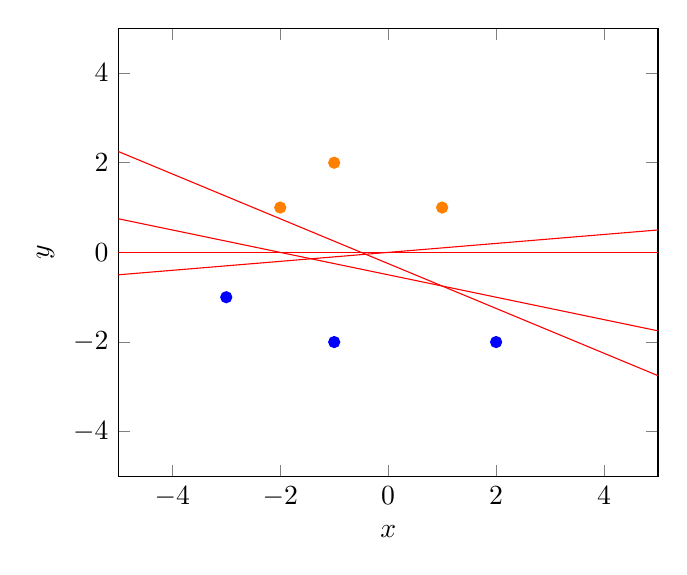
\begin{tikzpicture}

  \begin{axis}[xlabel = $x$, ylabel = $y$, xmin = -5.0, xmax = 5.0, ymin = -5.0, ymax = 5.0]
    
    \addplot[mark = *, , draw = none, color = orange] coordinates {(1,1)}; 
    \addplot[mark = *, , draw = none, color = orange] coordinates {(-1,2)}; 
    \addplot[mark = *, , draw = none, color = orange] coordinates {(-2,1)}; 

    \addplot[mark = *, , draw = none, color = blue] coordinates {(-1,-2)}; 
    \addplot[mark = *, , draw = none, color = blue] coordinates {(2,-2)}; 
    \addplot[mark = *, , draw = none, color = blue] coordinates {(-3,-1)}; 

    \addplot[color = red] {0};
    \addplot[color = red] {-0.25*x - 0.50};
    \addplot[color = red] {-0.50*x - 0.25};
    \addplot[color = red] {0.1*x};
    
    %\addplot[mark = *, , draw = none, color = red] coordinates {(-1,-1)};

  \end{axis}

\end{tikzpicture}
  \caption{Examples of separation lines for two-dimensional data.}
  \label{fig: perceptron}
\end{figure}

One can expect that the best separation hyperplane should be possible as far as possible from both testing samples. Intuitively, the ``real'' boundary separating classes (which is unknown) is located far from the center of training sets. This way, one may expect better classification of unusual testing points, so better generalization of the problem.

SVM guarantees (for linearly separable classes) finding the maximum-margin hyperplane. It can be easily extend for ``almost'' linearly separable classes, like those presented on Fig. \ref{fig: knnSepTrainSetOvr} (see Sec. \ref{sec: svmAlmost}). For classes linearly inseparable, {\it kernel trick} is used to transform feature space to higher dimension, where classes are linearly separable and maximum-margin hyperplane can be found (see Sec. \ref{sec: svmKernel}).

The task is ``easy'' - find the separation hyperplane and classification is straightforward.